\documentclass[a4paper]{book}
\usepackage{makeidx}
\usepackage{natbib}
\usepackage{graphicx}
\usepackage{multicol}
\usepackage{float}
\usepackage{listings}
\usepackage{color}
\usepackage{ifthen}
\usepackage[table]{xcolor}
\usepackage{textcomp}
\usepackage{alltt}
\usepackage{ifpdf}
\ifpdf
\usepackage[pdftex,
            pagebackref=true,
            colorlinks=true,
            linkcolor=blue,
            unicode
           ]{hyperref}
\else
\usepackage[ps2pdf,
            pagebackref=true,
            colorlinks=true,
            linkcolor=blue,
            unicode
           ]{hyperref}
\usepackage{pspicture}
\fi
\usepackage[utf8]{inputenc}
\usepackage{mathptmx}
\usepackage[scaled=.90]{helvet}
\usepackage{courier}
\usepackage{sectsty}
\usepackage[titles]{tocloft}
\usepackage{doxygen}
\lstset{language=C++,inputencoding=utf8,basicstyle=\footnotesize,breaklines=true,breakatwhitespace=true,tabsize=8,numbers=left }
\makeindex
\setcounter{tocdepth}{3}
\renewcommand{\footrulewidth}{0.4pt}
\renewcommand{\familydefault}{\sfdefault}
\hfuzz=15pt
\setlength{\emergencystretch}{15pt}
\hbadness=750
\tolerance=750
\begin{document}
\hypersetup{pageanchor=false,citecolor=blue}
\begin{titlepage}
\vspace*{7cm}
\begin{center}
{\Large cmake sample \\[1ex]\large 0.\-1 }\\
\vspace*{1cm}
{\large 作成: Doxygen 1.7.6.1}\\
\vspace*{0.5cm}
{\small Wed Jan 16 2013 22:34:09}\\
\end{center}
\end{titlepage}
\clearemptydoublepage
\pagenumbering{roman}
\tableofcontents
\clearemptydoublepage
\pagenumbering{arabic}
\hypersetup{pageanchor=true,citecolor=blue}
\chapter{構成索引}
\section{構成}
クラス、構造体、共用体、インタフェースの説明です。\begin{DoxyCompactList}
\item\contentsline{section}{\hyperlink{classDemoClass}{\-Demo\-Class} }{\pageref{classDemoClass}}{}
\item\contentsline{section}{\hyperlink{classSayClass}{\-Say\-Class} }{\pageref{classSayClass}}{}
\end{DoxyCompactList}

\chapter{ファイル索引}
\section{ファイル一覧}
これはファイル一覧です。\begin{DoxyCompactList}
\item\contentsline{section}{\-Demo\-Class/\hyperlink{DemoClass_8cpp}{\-Demo\-Class.\-cpp} }{\pageref{DemoClass_8cpp}}{}
\item\contentsline{section}{\-Demo\-Class/\hyperlink{DemoClass_8h}{\-Demo\-Class.\-h} }{\pageref{DemoClass_8h}}{}
\item\contentsline{section}{\-Main/\hyperlink{main_8cpp}{main.\-cpp} }{\pageref{main_8cpp}}{}
\item\contentsline{section}{\-Say\-Class/\hyperlink{SayClass_8cpp}{\-Say\-Class.\-cpp} }{\pageref{SayClass_8cpp}}{}
\item\contentsline{section}{\-Say\-Class/\hyperlink{SayClass_8h}{\-Say\-Class.\-h} }{\pageref{SayClass_8h}}{}
\end{DoxyCompactList}

\chapter{クラス}
\hypertarget{classDemoClass}{\section{クラス \-Demo\-Class}
\label{classDemoClass}\index{\-Demo\-Class@{\-Demo\-Class}}
}


{\ttfamily \#include $<$\-Demo\-Class.\-h$>$}



\-Demo\-Classのコラボレーション図
\nopagebreak
\begin{figure}[H]
\begin{center}
\leavevmode
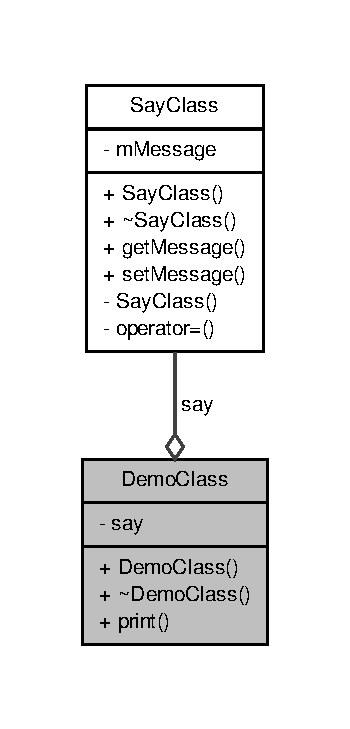
\includegraphics[width=168pt]{classDemoClass__coll__graph}
\end{center}
\end{figure}
\subsection*{\-Public メソッド}
\begin{DoxyCompactItemize}
\item 
\hyperlink{classDemoClass_ab232708c2e87c26b1292e55ad8a5a00f}{\-Demo\-Class} ()
\item 
\hyperlink{classDemoClass_ac22c3b34b51febc4c57e70f68c552da3}{$\sim$\-Demo\-Class} ()
\item 
void \hyperlink{classDemoClass_a6c357e6031ede08427a7cf9dc880477c}{print} ()
\end{DoxyCompactItemize}
\subsection*{\-Private 変数}
\begin{DoxyCompactItemize}
\item 
\hyperlink{classSayClass}{\-Say\-Class} \& \hyperlink{classDemoClass_aed27d0c4483b8a29069e2e90efb8ff12}{say}
\end{DoxyCompactItemize}


\subsection{説明}


 \-Demo\-Class.\-h の 3 行で定義されています。



\subsection{コンストラクタとデストラクタ}
\hypertarget{classDemoClass_ab232708c2e87c26b1292e55ad8a5a00f}{\index{\-Demo\-Class@{\-Demo\-Class}!\-Demo\-Class@{\-Demo\-Class}}
\index{\-Demo\-Class@{\-Demo\-Class}!DemoClass@{\-Demo\-Class}}
\subsubsection[{\-Demo\-Class}]{\setlength{\rightskip}{0pt plus 5cm}{\bf \-Demo\-Class\-::\-Demo\-Class} (
\begin{DoxyParamCaption}
{}
\end{DoxyParamCaption}
)}}\label{classDemoClass_ab232708c2e87c26b1292e55ad8a5a00f}


 \-Demo\-Class.\-cpp の 5 行で定義されています。

\hypertarget{classDemoClass_ac22c3b34b51febc4c57e70f68c552da3}{\index{\-Demo\-Class@{\-Demo\-Class}!$\sim$\-Demo\-Class@{$\sim$\-Demo\-Class}}
\index{$\sim$\-Demo\-Class@{$\sim$\-Demo\-Class}!DemoClass@{\-Demo\-Class}}
\subsubsection[{$\sim$\-Demo\-Class}]{\setlength{\rightskip}{0pt plus 5cm}{\bf \-Demo\-Class\-::$\sim$\-Demo\-Class} (
\begin{DoxyParamCaption}
{}
\end{DoxyParamCaption}
)}}\label{classDemoClass_ac22c3b34b51febc4c57e70f68c552da3}


 \-Demo\-Class.\-cpp の 10 行で定義されています。



参照先 say.



\subsection{関数}
\hypertarget{classDemoClass_a6c357e6031ede08427a7cf9dc880477c}{\index{\-Demo\-Class@{\-Demo\-Class}!print@{print}}
\index{print@{print}!DemoClass@{\-Demo\-Class}}
\subsubsection[{print}]{\setlength{\rightskip}{0pt plus 5cm}void {\bf \-Demo\-Class\-::print} (
\begin{DoxyParamCaption}
{}
\end{DoxyParamCaption}
)}}\label{classDemoClass_a6c357e6031ede08427a7cf9dc880477c}


 \-Demo\-Class.\-cpp の 14 行で定義されています。



参照先 \-Say\-Class\-::get\-Message(), say, と \-Say\-Class\-::set\-Message().



参照元 main().



関数の呼び出しグラフ\-:
\nopagebreak
\begin{figure}[H]
\begin{center}
\leavevmode
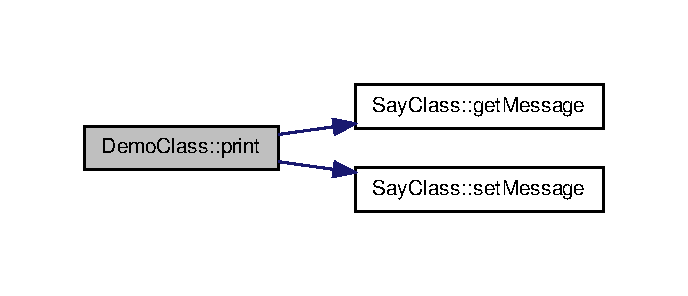
\includegraphics[width=330pt]{classDemoClass_a6c357e6031ede08427a7cf9dc880477c_cgraph}
\end{center}
\end{figure}




呼出しグラフ\-:
\nopagebreak
\begin{figure}[H]
\begin{center}
\leavevmode
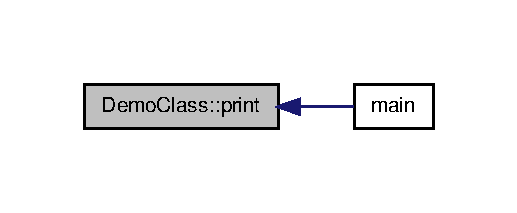
\includegraphics[width=248pt]{classDemoClass_a6c357e6031ede08427a7cf9dc880477c_icgraph}
\end{center}
\end{figure}




\subsection{変数}
\hypertarget{classDemoClass_aed27d0c4483b8a29069e2e90efb8ff12}{\index{\-Demo\-Class@{\-Demo\-Class}!say@{say}}
\index{say@{say}!DemoClass@{\-Demo\-Class}}
\subsubsection[{say}]{\setlength{\rightskip}{0pt plus 5cm}{\bf \-Say\-Class}\& {\bf \-Demo\-Class\-::say}\hspace{0.3cm}{\ttfamily  \mbox{[}private\mbox{]}}}}\label{classDemoClass_aed27d0c4483b8a29069e2e90efb8ff12}


 \-Demo\-Class.\-h の 9 行で定義されています。



参照元 print(), と $\sim$\-Demo\-Class().



このクラスの説明は次のファイルから生成されました\-:\begin{DoxyCompactItemize}
\item 
\-Demo\-Class/\hyperlink{DemoClass_8h}{\-Demo\-Class.\-h}\item 
\-Demo\-Class/\hyperlink{DemoClass_8cpp}{\-Demo\-Class.\-cpp}\end{DoxyCompactItemize}

\hypertarget{classSayClass}{\section{クラス \-Say\-Class}
\label{classSayClass}\index{\-Say\-Class@{\-Say\-Class}}
}


{\ttfamily \#include $<$\-Say\-Class.\-h$>$}

\subsection*{\-Public メソッド}
\begin{DoxyCompactItemize}
\item 
\hyperlink{classSayClass_ac9fb8db5cd217f8e5123fbe8043f9007}{\-Say\-Class} ()
\begin{DoxyCompactList}\small\item\em \-Constractor. \end{DoxyCompactList}\item 
\hyperlink{classSayClass_a54d89f97051256c5ba31c19e03ed3418}{$\sim$\-Say\-Class} ()
\begin{DoxyCompactList}\small\item\em \-Destractor. \end{DoxyCompactList}\item 
string \hyperlink{classSayClass_a619e0ee356f9c04aa79ef11a8a3965fd}{get\-Message} () const 
\begin{DoxyCompactList}\small\item\em \-Get \-Say \-Message. \end{DoxyCompactList}\item 
void \hyperlink{classSayClass_afb4d7ea98d95e9b9eba553cc8aca4dd7}{set\-Message} (const string a\-Message)
\begin{DoxyCompactList}\small\item\em \-Set \-Say \-Message. \end{DoxyCompactList}\end{DoxyCompactItemize}
\subsection*{\-Private メソッド}
\begin{DoxyCompactItemize}
\item 
\hyperlink{classSayClass_acf487fb2d4c4d76cd509212b42170763}{\-Say\-Class} (const \hyperlink{classSayClass}{\-Say\-Class} \&a\-Obj)
\begin{DoxyCompactList}\small\item\em \-Disable \-Copy \-Constractor. \end{DoxyCompactList}\item 
void \hyperlink{classSayClass_a02e6b50715d6f1a0633c6436d1779659}{operator=} (const \hyperlink{classSayClass}{\-Say\-Class} \&a\-Obj)
\end{DoxyCompactItemize}
\subsection*{\-Private 変数}
\begin{DoxyCompactItemize}
\item 
string \hyperlink{classSayClass_ae8e574040647db1b0f289f3aec5566ee}{m\-Message}
\begin{DoxyCompactList}\small\item\em \-Message. \end{DoxyCompactList}\end{DoxyCompactItemize}


\subsection{説明}


 \-Say\-Class.\-h の 7 行で定義されています。



\subsection{コンストラクタとデストラクタ}
\hypertarget{classSayClass_ac9fb8db5cd217f8e5123fbe8043f9007}{\index{\-Say\-Class@{\-Say\-Class}!\-Say\-Class@{\-Say\-Class}}
\index{\-Say\-Class@{\-Say\-Class}!SayClass@{\-Say\-Class}}
\subsubsection[{\-Say\-Class}]{\setlength{\rightskip}{0pt plus 5cm}{\bf \-Say\-Class\-::\-Say\-Class} (
\begin{DoxyParamCaption}
{}
\end{DoxyParamCaption}
)}}\label{classSayClass_ac9fb8db5cd217f8e5123fbe8043f9007}


\-Constractor. 



 \-Say\-Class.\-cpp の 14 行で定義されています。

\hypertarget{classSayClass_a54d89f97051256c5ba31c19e03ed3418}{\index{\-Say\-Class@{\-Say\-Class}!$\sim$\-Say\-Class@{$\sim$\-Say\-Class}}
\index{$\sim$\-Say\-Class@{$\sim$\-Say\-Class}!SayClass@{\-Say\-Class}}
\subsubsection[{$\sim$\-Say\-Class}]{\setlength{\rightskip}{0pt plus 5cm}{\bf \-Say\-Class\-::$\sim$\-Say\-Class} (
\begin{DoxyParamCaption}
{}
\end{DoxyParamCaption}
)}}\label{classSayClass_a54d89f97051256c5ba31c19e03ed3418}


\-Destractor. 



 \-Say\-Class.\-cpp の 22 行で定義されています。

\hypertarget{classSayClass_acf487fb2d4c4d76cd509212b42170763}{\index{\-Say\-Class@{\-Say\-Class}!\-Say\-Class@{\-Say\-Class}}
\index{\-Say\-Class@{\-Say\-Class}!SayClass@{\-Say\-Class}}
\subsubsection[{\-Say\-Class}]{\setlength{\rightskip}{0pt plus 5cm}{\bf \-Say\-Class\-::\-Say\-Class} (
\begin{DoxyParamCaption}
\item[{const {\bf \-Say\-Class} \&}]{a\-Obj}
\end{DoxyParamCaption}
)\hspace{0.3cm}{\ttfamily  \mbox{[}private\mbox{]}}}}\label{classSayClass_acf487fb2d4c4d76cd509212b42170763}


\-Disable \-Copy \-Constractor. 



\subsection{関数}
\hypertarget{classSayClass_a619e0ee356f9c04aa79ef11a8a3965fd}{\index{\-Say\-Class@{\-Say\-Class}!get\-Message@{get\-Message}}
\index{get\-Message@{get\-Message}!SayClass@{\-Say\-Class}}
\subsubsection[{get\-Message}]{\setlength{\rightskip}{0pt plus 5cm}string {\bf \-Say\-Class\-::get\-Message} (
\begin{DoxyParamCaption}
{}
\end{DoxyParamCaption}
) const}}\label{classSayClass_a619e0ee356f9c04aa79ef11a8a3965fd}


\-Get \-Say \-Message. 



 \-Say\-Class.\-cpp の 29 行で定義されています。



参照先 m\-Message.



参照元 \-Demo\-Class\-::print().



呼出しグラフ\-:
\nopagebreak
\begin{figure}[H]
\begin{center}
\leavevmode
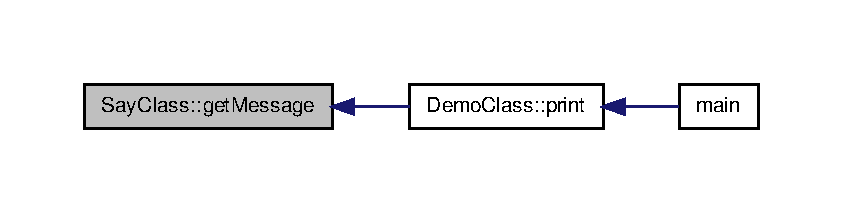
\includegraphics[width=350pt]{classSayClass_a619e0ee356f9c04aa79ef11a8a3965fd_icgraph}
\end{center}
\end{figure}


\hypertarget{classSayClass_a02e6b50715d6f1a0633c6436d1779659}{\index{\-Say\-Class@{\-Say\-Class}!operator=@{operator=}}
\index{operator=@{operator=}!SayClass@{\-Say\-Class}}
\subsubsection[{operator=}]{\setlength{\rightskip}{0pt plus 5cm}void \-Say\-Class\-::operator= (
\begin{DoxyParamCaption}
\item[{const {\bf \-Say\-Class} \&}]{a\-Obj}
\end{DoxyParamCaption}
)\hspace{0.3cm}{\ttfamily  \mbox{[}private\mbox{]}}}}\label{classSayClass_a02e6b50715d6f1a0633c6436d1779659}
\hypertarget{classSayClass_afb4d7ea98d95e9b9eba553cc8aca4dd7}{\index{\-Say\-Class@{\-Say\-Class}!set\-Message@{set\-Message}}
\index{set\-Message@{set\-Message}!SayClass@{\-Say\-Class}}
\subsubsection[{set\-Message}]{\setlength{\rightskip}{0pt plus 5cm}void {\bf \-Say\-Class\-::set\-Message} (
\begin{DoxyParamCaption}
\item[{const string}]{a\-Message}
\end{DoxyParamCaption}
)}}\label{classSayClass_afb4d7ea98d95e9b9eba553cc8aca4dd7}


\-Set \-Say \-Message. 

\-:a\-Message 

 \-Say\-Class.\-cpp の 39 行で定義されています。



参照先 m\-Message.



参照元 \-Demo\-Class\-::print().



呼出しグラフ\-:
\nopagebreak
\begin{figure}[H]
\begin{center}
\leavevmode
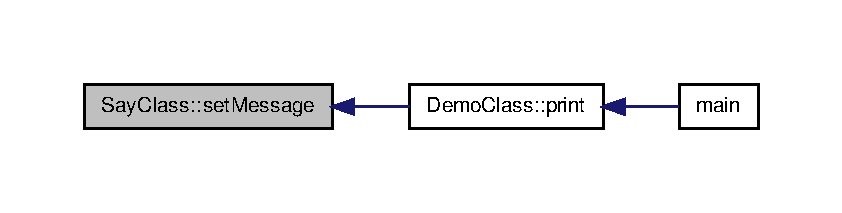
\includegraphics[width=350pt]{classSayClass_afb4d7ea98d95e9b9eba553cc8aca4dd7_icgraph}
\end{center}
\end{figure}




\subsection{変数}
\hypertarget{classSayClass_ae8e574040647db1b0f289f3aec5566ee}{\index{\-Say\-Class@{\-Say\-Class}!m\-Message@{m\-Message}}
\index{m\-Message@{m\-Message}!SayClass@{\-Say\-Class}}
\subsubsection[{m\-Message}]{\setlength{\rightskip}{0pt plus 5cm}string {\bf \-Say\-Class\-::m\-Message}\hspace{0.3cm}{\ttfamily  \mbox{[}private\mbox{]}}}}\label{classSayClass_ae8e574040647db1b0f289f3aec5566ee}


\-Message. 



 \-Say\-Class.\-h の 29 行で定義されています。



参照元 get\-Message(), と set\-Message().



このクラスの説明は次のファイルから生成されました\-:\begin{DoxyCompactItemize}
\item 
\-Say\-Class/\hyperlink{SayClass_8h}{\-Say\-Class.\-h}\item 
\-Say\-Class/\hyperlink{SayClass_8cpp}{\-Say\-Class.\-cpp}\end{DoxyCompactItemize}

\chapter{ファイル}
\hypertarget{DemoClass_8cpp}{\section{\-Demo\-Class/\-Demo\-Class.cpp}
\label{DemoClass_8cpp}\index{\-Demo\-Class/\-Demo\-Class.\-cpp@{\-Demo\-Class/\-Demo\-Class.\-cpp}}
}
{\ttfamily \#include $<$stdio.\-h$>$}\*
{\ttfamily \#include \char`\"{}\-Demo\-Class.\-h\char`\"{}}\*
\-Demo\-Class.\-cppのインクルード依存関係図
\nopagebreak
\begin{figure}[H]
\begin{center}
\leavevmode
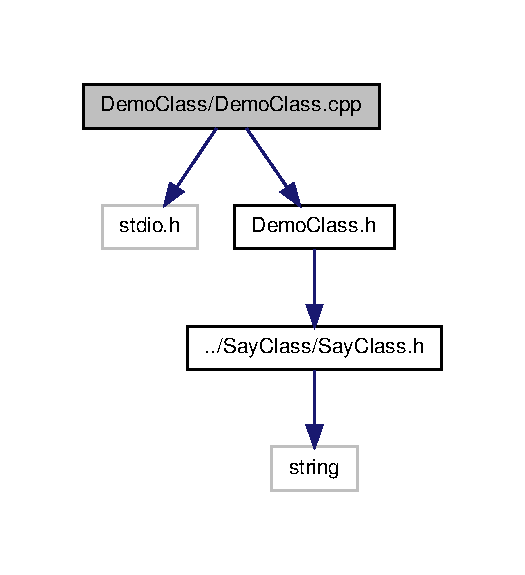
\includegraphics[width=252pt]{DemoClass_8cpp__incl}
\end{center}
\end{figure}

\hypertarget{DemoClass_8h}{\section{\-Demo\-Class/\-Demo\-Class.h}
\label{DemoClass_8h}\index{\-Demo\-Class/\-Demo\-Class.\-h@{\-Demo\-Class/\-Demo\-Class.\-h}}
}
{\ttfamily \#include \char`\"{}../\-Say\-Class/\-Say\-Class.\-h\char`\"{}}\*
\-Demo\-Class.\-hのインクルード依存関係図
\nopagebreak
\begin{figure}[H]
\begin{center}
\leavevmode
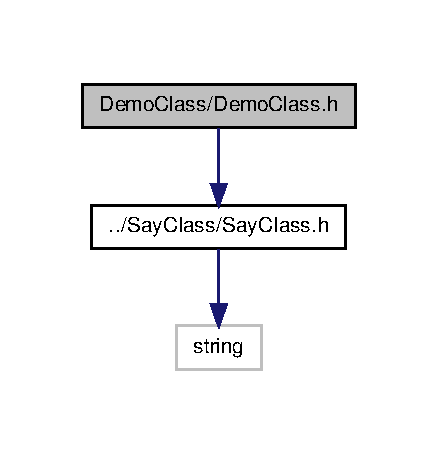
\includegraphics[width=210pt]{DemoClass_8h__incl}
\end{center}
\end{figure}
このグラフは、どのファイルから直接、間接的にインクルードされているかを示しています。
\nopagebreak
\begin{figure}[H]
\begin{center}
\leavevmode
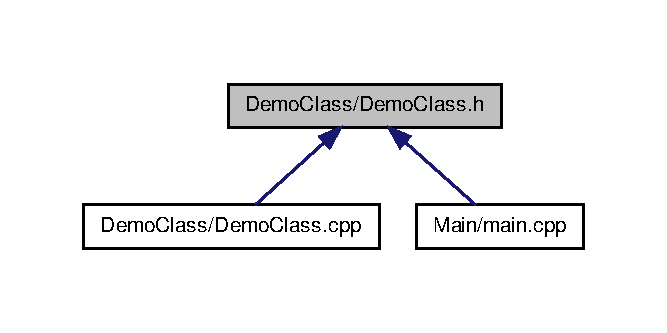
\includegraphics[width=320pt]{DemoClass_8h__dep__incl}
\end{center}
\end{figure}
\subsection*{構成}
\begin{DoxyCompactItemize}
\item 
class \hyperlink{classDemoClass}{\-Demo\-Class}
\end{DoxyCompactItemize}

\hypertarget{main_8cpp}{\section{\-Main/main.cpp}
\label{main_8cpp}\index{\-Main/main.\-cpp@{\-Main/main.\-cpp}}
}
{\ttfamily \#include $<$stdio.\-h$>$}\*
{\ttfamily \#include \char`\"{}../\-Demo\-Class/\-Demo\-Class.\-h\char`\"{}}\*
main.\-cppのインクルード依存関係図
\nopagebreak
\begin{figure}[H]
\begin{center}
\leavevmode
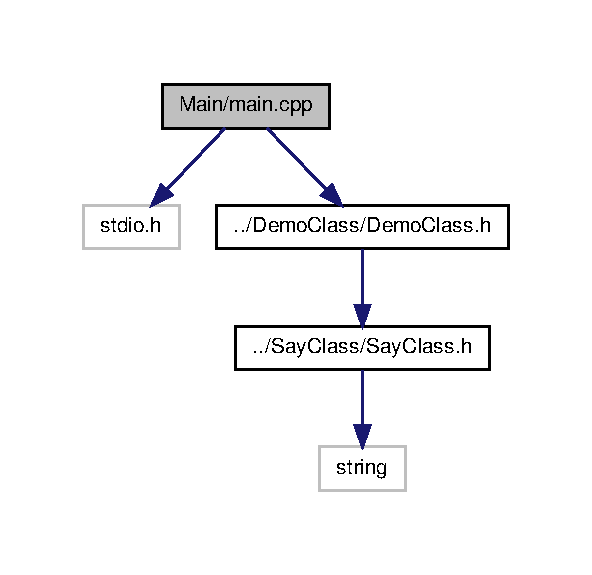
\includegraphics[width=284pt]{main_8cpp__incl}
\end{center}
\end{figure}
\subsection*{関数}
\begin{DoxyCompactItemize}
\item 
int \hyperlink{main_8cpp_abf9e6b7e6f15df4b525a2e7705ba3089}{main} (int argc, char const $\ast$argv\mbox{[}$\,$\mbox{]})
\end{DoxyCompactItemize}


\subsection{関数}
\hypertarget{main_8cpp_abf9e6b7e6f15df4b525a2e7705ba3089}{\index{main.\-cpp@{main.\-cpp}!main@{main}}
\index{main@{main}!main.cpp@{main.\-cpp}}
\subsubsection[{main}]{\setlength{\rightskip}{0pt plus 5cm}int {\bf main} (
\begin{DoxyParamCaption}
\item[{int}]{argc, }
\item[{char const $\ast$}]{argv\mbox{[}$\,$\mbox{]}}
\end{DoxyParamCaption}
)}}\label{main_8cpp_abf9e6b7e6f15df4b525a2e7705ba3089}


 main.\-cpp の 5 行で定義されています。



参照先 \-Demo\-Class\-::print().



関数の呼び出しグラフ\-:
\nopagebreak
\begin{figure}[H]
\begin{center}
\leavevmode
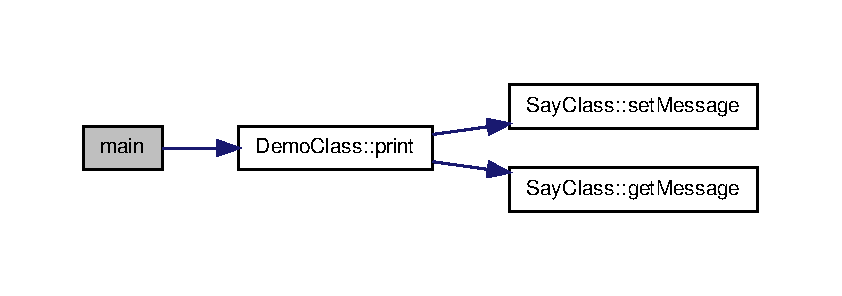
\includegraphics[width=350pt]{main_8cpp_abf9e6b7e6f15df4b525a2e7705ba3089_cgraph}
\end{center}
\end{figure}



\hypertarget{SayClass_8cpp}{\section{\-Say\-Class/\-Say\-Class.cpp}
\label{SayClass_8cpp}\index{\-Say\-Class/\-Say\-Class.\-cpp@{\-Say\-Class/\-Say\-Class.\-cpp}}
}
{\ttfamily \#include \char`\"{}\-Say\-Class.\-h\char`\"{}}\*
\-Say\-Class.\-cppのインクルード依存関係図
\nopagebreak
\begin{figure}[H]
\begin{center}
\leavevmode
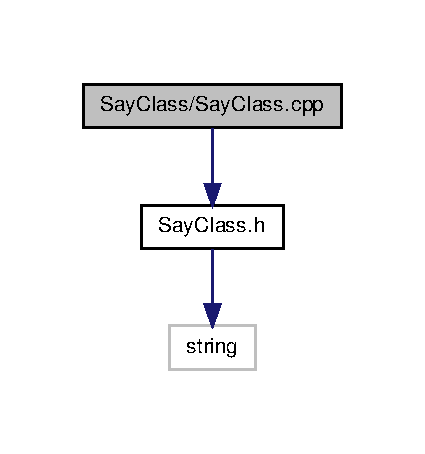
\includegraphics[width=204pt]{SayClass_8cpp__incl}
\end{center}
\end{figure}


\subsection{説明}
\begin{DoxyAuthor}{作者}
\-Masashi \-Kayahara 
\end{DoxyAuthor}
\begin{DoxyVersion}{バージョン}
0.\-1 
\end{DoxyVersion}
\begin{DoxyDate}{日付}
2011-\/12-\/11 
\end{DoxyDate}


 \hyperlink{SayClass_8cpp_source}{\-Say\-Class.\-cpp} で定義されています。


\hypertarget{SayClass_8h}{\section{\-Say\-Class/\-Say\-Class.h}
\label{SayClass_8h}\index{\-Say\-Class/\-Say\-Class.\-h@{\-Say\-Class/\-Say\-Class.\-h}}
}
{\ttfamily \#include $<$string$>$}\*
\-Say\-Class.\-hのインクルード依存関係図
\nopagebreak
\begin{figure}[H]
\begin{center}
\leavevmode
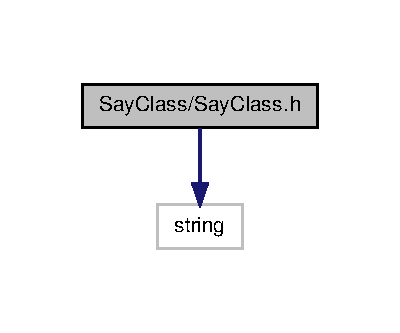
\includegraphics[width=192pt]{SayClass_8h__incl}
\end{center}
\end{figure}
このグラフは、どのファイルから直接、間接的にインクルードされているかを示しています。
\nopagebreak
\begin{figure}[H]
\begin{center}
\leavevmode
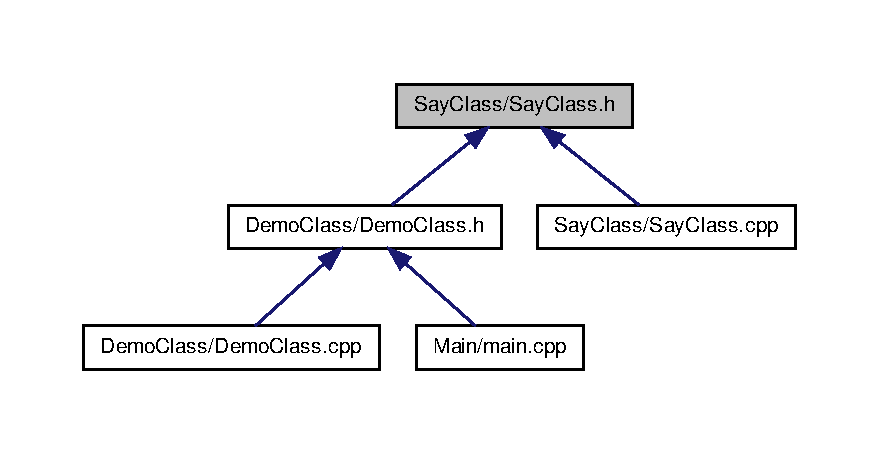
\includegraphics[width=350pt]{SayClass_8h__dep__incl}
\end{center}
\end{figure}
\subsection*{構成}
\begin{DoxyCompactItemize}
\item 
class \hyperlink{classSayClass}{\-Say\-Class}
\end{DoxyCompactItemize}

\printindex
\end{document}
